\chapter{Исследование свойств применяемых стёкол}

В данной главе представлены результаты исследований состава стёкол марок
Borofloat~33, Corning~7740, ЛК5 и~Hoya~SD\nb-2.
Затем описана процедура определения их температурных коэффициентов линейного
расширения. Полученные значения аппроксимированы полиномиальными функциями
и~сравнены с данными производителей.

\section{Литературные данные по маркам стекла, совместимым с~анодной посадкой} \label{GlassInfoOffic}

\subsection{Температурная зависимость коэффициентов теплового расширения}

Для описания температурной зависимости температурных коэффициентов линейного расширения используется приближение в виде полиномов:
\begin{equation*}
    P(T) = a + b \cdot T + c \cdot T^2 + d \cdot T^3 + e \cdot T^4 + f \cdot T^5,
\end{equation*}
где $a$, $b$, $c$, $d$, $e$, $f$ "--- коэффициенты полинома. Подобным представлением удобно пользоваться как в аналитических моделях, так и при применении конечноэлементных вычислительных комплексов.

Коэффициенты полиномов для рассматриваемых стёкол с диапазоном применимости сведены в Таблицу~\ref{tab:glass_polynoms_official}. Производители не приводят данных по~температурной зависимости температурных коэффициентов линейного расширения своих стёкол в аналитической форме. Поэтому, при наличии среди данных производителей графиков зависимостей, полиномиальные зависимости получались аппроксимацией точек графиков.

\begin{table} [!ht]
    \centering%
	\caption{Коэффициенты полиномов $\alpha (T)$, 1/K, на основании данных производителей стёкол}%
	\label{tab:glass_polynoms_official}% label всегда желательно идти после caption
    \tabulinesep=2.1mm
	\begin{SingleSpace}
	\begin{tabu} to \textwidth {@{}
	X[l,m]
	S[table-format=-1.3]
	S[table-format=-1.3]
	S[table-format=-2.3]
	S[table-format=-2.3]
	S[table-format=-1.3]
	S[table-format=-1.3]
	>{\raggedleft}m{0.9cm}@{---}>{\raggedright\arraybackslash}m{0.9cm}%
	@{}}
        \toprule     %%% верхняя линейка
        {Марка стекла} &
        {$a, 10^{-6}$} &
        {$b, 10^{-8}$} &
        {$c, 10^{-11}$}&
        {$d, 10^{-14}$}&
        {$e, 10^{-16}$} &
        {$f, 10^{-19}$} &
        \multicolumn{2}{>{\centering\arraybackslash}m{2.3cm}@{}}{Диапа\-зон, K}\\
        \midrule
        Corning 7740 &
        6,975 &
        -5,405 &
        28,730 &
        -69,350 &
        7,694 &
        -3,167 &
        323&673\\
        Schott Borofloat~33 &
        -1.195 &
        3.574 &
        -11.760 &
        20.540 &
        -1.919 &
        0.748 &
        153&773\\
        ЛК5 & 2.737 & 0.222 & 0.000 & 0.000 & 0.000 & 0.000 & 213&393\\
        Hoya SD\nobreakdash-2 &
        -3,382 &
        2,750 &
        -2,723 &
        -2,496 &
        0,628 &
        -0,296 &
        373&773\\
        Asahi SW\nobreakdash-YY &
        -3,879 &
        6,526 &
        -27,290 &
        59,860 &
        -6,408 &
        2,638 &
        303&723\\
        \bottomrule %%% нижняя линейка
	\end{tabu}%
	\end{SingleSpace}
\end{table}

Зависимости ТКЛР от температуры для стёкол марок SD\nb-2 и SW\nb-YY получены из графиков в~\cite{SD_2_properties} и~\cite{swyy_properties}, соответственно.
Зависимости ТКЛР от~температуры для стёкол марок 7740 и Borofloat~33 получены расчётным путём из~графиков температурных зависимостей относительного удлинения от~температуры, приведённых в~\cite{corning7740_wafersheet} и~\cite{bf33_properties}.
Расчёт полиномиальной зависимости ТКЛР для стекла марки ЛК5 был проведён на основании данных по средним \mbox{ТКЛР} в двух температурных диапазонах, указанных производителем~\cite{LK5_properties}, исходя из предположения, что температурный ход значения коэффициента в~области «нормального» состояния стёкол, от минус 120~{\textdegree}C до температуры нижней границы зоны отжига, практически выражается линейным уравнением~\cites[180]{Mazurin1969_Tepl_rassh_stekla}.

На основании тех же литературных источников в Таблице~\ref{tab:glass_cteavg_official} представлены средние ТКЛР для рассмотренных стёкол.

\begin{table} [!htb]
    \centering%
    \parbox{0.8\textwidth}{
	\caption{Средние ТКЛР для стёкол по литературным данным}%
	\label{tab:glass_cteavg_official}% label всегда желательно идти после caption
	}
    \tabulinesep=1.8mm
	\begin{SingleSpace}
	\begin{tabu} to 0.8\textwidth {@{}
	X[l]
	>{\raggedleft}m{0.9cm}@{---}>{\raggedright}m{0.9cm}%
	S[table-format=1.2]
	@{}}
        \toprule     %%% верхняя линейка
        {Марка стекла} &
        \multicolumn{2}{>{\centering}m{3.0cm}}{Диапа\-зон,~{\textdegree}C} &
        {Средний ТКЛР, 10\textsuperscript{$-$6}~{\textdegree}C\textsuperscript{$-$1}}\\
        \midrule
        Corning 7740 &
        0&300 &
        3,25\\
        Schott Borofloat~33 &
        20&300 &
        3,25\\
        \multirow{2}{*}{ЛК5} &
        $-$60&20 &
        3,30\\
         &
        20&120 &
        3,50\\
        Hoya SD\nobreakdash-2 &
        20&300 &
        3,20\\
        Asahi SW\nobreakdash-YY &
        30&300 &
        3,30\\
        \bottomrule %%% нижняя линейка
	\end{tabu}%
	\end{SingleSpace}
\end{table}

На Рисунке~\ref{fig:cte_offic}
приведены графики зависимостей ТКЛР от температуры из Таблицы~\ref{tab:glass_polynoms_official}.

\begin{figure}[!htb]
    \centering
    \begingroup%
      \makeatletter%
      \providecommand\color[2][]{%
        \errmessage{(Inkscape) Color is used for the text in Inkscape, but the package 'color.sty' is not loaded}%
        \renewcommand\color[2][]{}%
      }%
      \providecommand\transparent[1]{%
        \errmessage{(Inkscape) Transparency is used (non-zero) for the text in Inkscape, but the package 'transparent.sty' is not loaded}%
        \renewcommand\transparent[1]{}%
      }%
      \providecommand\rotatebox[2]{#2}%
      \ifx\svgwidth\undefined%
        \setlength{\unitlength}{0.6\textwidth}%
        \ifx\svgscale\undefined%
          \relax%
        \else%
          \setlength{\unitlength}{\unitlength * \real{\svgscale}}%
        \fi%
      \else%
        \setlength{\unitlength}{\svgwidth}%
      \fi%
      \global\let\svgwidth\undefined%
      \global\let\svgscale\undefined%
      \makeatother%
      \begin{picture}(1,0.91245741)%
        \put(0,0){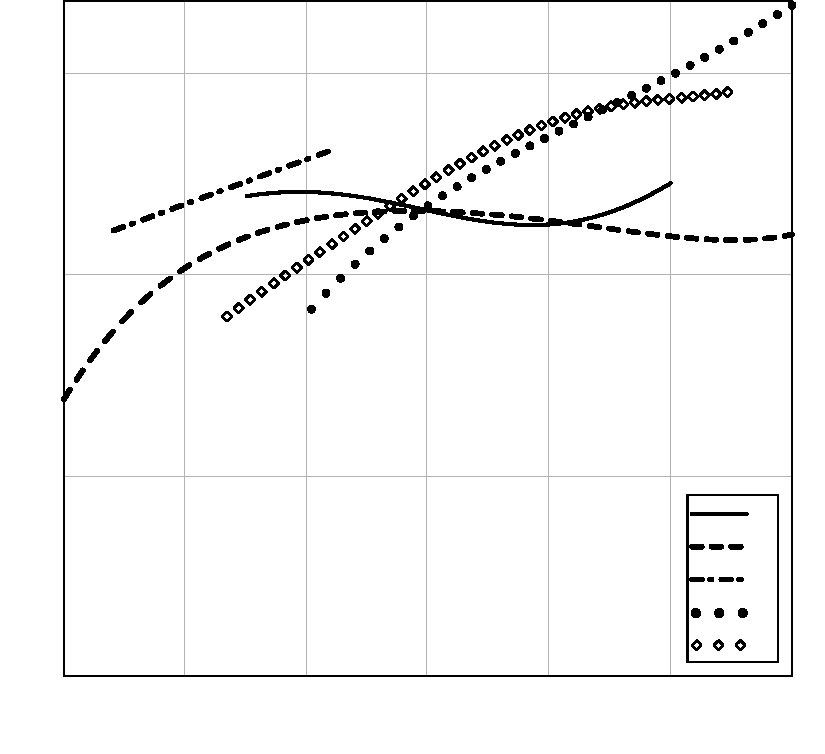
\includegraphics[width=\unitlength]{cte_offic}}%
        \put(0.911,0.279){\color[named]{black}\makebox(0,0)[lb]{\smash{\textsl{1}}}}%
        \put(0.911,0.239){\color[named]{black}\makebox(0,0)[lb]{\smash{\textsl{2}}}}%
        \put(0.911,0.199){\color[named]{black}\makebox(0,0)[lb]{\smash{\textsl{3}}}}%
        \put(0.911,0.159){\color[named]{black}\makebox(0,0)[lb]{\smash{\textsl{4}}}}%
        \put(0.911,0.120){\color[named]{black}\makebox(0,0)[lb]{\smash{\textsl{5}}}}%
        \put(0.04942711,0.05401028){\color[named]{black}\makebox(0,0)[lb]{\smash{$-$100}}}%
        \put(0.22365622,0.05401028){\color[named]{black}\makebox(0,0)[lb]{\smash{0}}}%
        \put(0.3564527,0.05401028){\color[named]{black}\makebox(0,0)[lb]{\smash{100}}}%
        \put(0.50245287,0.05401028){\color[named]{black}\makebox(0,0)[lb]{\smash{200}}}%
        \put(0.65042609,0.05401028){\color[named]{black}\makebox(0,0)[lb]{\smash{300}}}%
        \put(0.79839931,0.05401028){\color[named]{black}\makebox(0,0)[lb]{\smash{400}}}%
        \put(0.05427861,0.32142437){\color[named]{black}\makebox(0,0)[lb]{\smash{2}}}%
        \put(0.05360429,0.56622527){\color[named]{black}\makebox(0,0)[lb]{\smash{3}}}%
        \put(0.05448614,0.81087425){\color[named]{black}\makebox(0,0)[lb]{\smash{4}}}%
        \put(0.02458798,0.47333211){\color[named]{black}\rotatebox{90}{\makebox(0,0)[b]{\smash{$\alpha$, 10\textsuperscript{$-$6}~{\textdegree}C\textsuperscript{$-$1}}}}}%
        \put(0.94814372,0.05401028){\color[named]{black}\makebox(0,0)[lb]{\smash{500}}}%
        \put(0.05088957,0.08264282){\color[named]{black}\makebox(0,0)[lb]{\smash{1}}}%
        \put(0.51958915,0.0075735){\color[named]{black}\makebox(0,0)[b]{\smash{$T$,~{\textdegree}C}}}%
      \end{picture}%
    \endgroup%

    \caption{Зависимости температурных коэффициентов линейного расширения от температуры для нескольких марок стекла и кремния:}
    \label{fig:cte_offic}
    \textsl{1} "--- Corning 7740,  \textsl{2} "--- Schott Borofloat 33,  \textsl{3} "--- ЛК5,  \textsl{4} "--- Hoya~SD-2,  \textsl{5}~---~Asahi~SW\nb-YY%
\end{figure}

\subsection{Упругие свойства}

В Таблице~\ref{table_glass_elasticity} приведены упругие свойства (модуль Юнга, \(E\), ГПа, и коэффициент Пуассона,  \(\mu\))  стёкол Hoya SD\nobreakdash-2~\cite{SD_2_properties}, Asahi SW\nobreakdash-YY~\cite{swyy_properties}, Corning~7740~\cite{corning7740_wafersheet}, Schott Borofloat~33~\cite{bf33_properties} и ЛК5~\cite{LK5_properties}.

\begin{table} [!htb]%
    \centering
    \parbox{0.5\textwidth}{
    	\caption{Упругие свойства рассматриваемых марок стёкол}%
    	\label{table_glass_elasticity}% label всегда желательно идти после caption
	}
    \renewcommand{\arraystretch}{1.15}%% Увеличение расстояния между рядами, для улучшения восприятия.
	\def\tabularxcolumn#1{m{#1}}
    \sisetup{round-mode = places}
	\begin{SingleSpace}
	\begin{tabularx}{0.5\textwidth}{@{}
	>{\raggedright}X
	S[round-precision = 2]
	S[round-precision = 3]
	@{}}
        \toprule     %%% верхняя линейка
        {Марка стекла} &
        {$E$, ГПa} &
        {$\mu$}\\
        \midrule %%% тонкий разделитель. Отделяет названия столбцов. Обязателен по ГОСТ 2.105 пункт 4.4.5

        Corning 7740 &
        62,75 &
        0,2\\
        Schott Borofloat 33 &
        64,0 &
        0,2\\
        ЛК5 &
        68,45 &
        0,184\\
        Hoya~SD-2 &
        86,89 &
        0,244 \\
        Asahi SW-YY &
        82,0 &
        0,2\\
        \bottomrule %%% нижняя линейка
	\end{tabularx}%
	\end{SingleSpace}
\end{table}

\section{Исследование состава стёкол}

<<Рентгеновская фотоэлектронная спектроскопия (РФЭС) "--- количественный спектроскопический метод исследования элементного состава, эмпирической формулы, химического и электронного состояния атомов, присутствующих в материале. Он основан на явлении внешнего фотоэффекта. Спектры РФЭС получают облучением материала пучком рентгеновских лучей с регистрацией зависимости количества испускаемых электронов
от~их~кинетической энергии. Исследуемые электроны испускаются верхним слоем исследуемого материала толщиной от 1 до 10 нм. РФЭС проводится
в~сверхвысоком вакууме>>~\cite{wiki_arxps}.

<<РФЭС "--- метод химического анализа поверхности, который может быть использован для анализа химического состояния материала как в его первоначальном состоянии, так и после некоторой обработки, например скола, разреза или очистки в воздухе или сверхвысоком вакууме для исследования внутреннего химического состава образца, облучения высокоэнергетическим пучком ионов для очистки поверхности от загрязнений, нагрева образца, чтобы изучить изменения вследствие нагревания, помещения в атмосферу реактивного газа или раствора, облучения ионами с целью их внедрения, облучения ультрафиолетовым светом>>~\cite{wiki_arxps}.

На установке Theta Probe {Angle-Resolved} {X-ray} Photoelectron Spectrometer (ARXPS) System методом рентгеновской фотоэлектронной спектроскопии были проведены измерения образцов стёкол марок Borofloat~33, Corning~7740, ЛК5 и~Hoya~SD\nb-2.
Измерения проводились
научным сотрудником ФГУП <<ВНИИА им.~Н.\,Л.~Духова>>
А.\:Ю.~Переяславцевым.
Полученный химический поэлементный состав приведён Таблице~\ref{tab:results_arxps_glass}.

\begin{table} [!ht]
    \centering%
    \parbox{0.8\textwidth}{
    	\caption{Результаты измерения химического состава стёкол}%
    	\label{tab:results_arxps_glass}% label всегда желательно идти после caption
	}
    \renewcommand{\arraystretch}{1.3}%% Увеличение расстояния между рядами, для улучшения восприятия.
    \begin{SingleSpace}
    \begin{tabularx}{0.8\textwidth}{@{}
    >{\raggedright}X
    llllllll@{}}
    \toprule
        \multirow{2}{*}{Марка стекла}
        &
        \multicolumn{8}{c}{Компоненты стекла, ат.~\%} \\
    \cmidrule(l){2-9}
%        Марка стекла
        & O & Si & B & Al & Na & K & Mg & Zn \\
    \midrule
        Borofloat 33 & 64,44 &  30,60 &  3,37 &   1,12 &   0,33 &  0,14 &   0,00 &   0,00 \\
        Corning 7740 & 63,68 &  29,20 &  5,24 &   1,26 &   0,47 &  0,15 &   0,00 &   0,00 \\
        ЛК5          & 63,19 &  31,28 &  2,55 &   1,34 &   0,93 &  0,07 &   0,64 &   0,00 \\
        Hoya SD\nb-2 & 63,59 &  23,72 &  1,11 &   9,29 &   0,56 &  0,12 &   0,95 &   0,67 \\
    \bottomrule %%% нижняя линейка
	\end{tabularx}%
    \end{SingleSpace}
\end{table}

Для удобства сравнения с данными литературных источников был проведён пересчёт результатов из Таблицы~\ref{tab:results_arxps_glass} в формат оксидного состава с допущением о простом строении оксидов.
Описание процедуры пересчёта приведено в~подразделе~\ref{GlassCompositionProgram}.
Результат пересчёта приведён в Таблице~\ref{tab:glass_oxides_calc}.

\begin{table} [!ht]
    \centering%
    \parbox{0.8\textwidth}{
    	\caption{Химический состав стёкол, пересчитанный в оксидной форме}%
    	\label{tab:glass_oxides_calc}% label всегда желательно идти после caption
	}
    \renewcommand{\arraystretch}{1.3}%% Увеличение расстояния между рядами, для улучшения восприятия.
    \sisetup{
        table-number-alignment = center,
        table-text-alignment = center,
        table-format=2.1,
        round-mode = places,
        round-precision = 1
    }%
    \begin{SingleSpace}
    \begin{tabularx}{0.8\textwidth}{@{}
    >{\raggedright}X
    SSSSSSS@{}}
    \toprule
        \multirow{2}{*}{Марка стекла}
        &
        \multicolumn{7}{c}{Оксидный состав, вес.~\%} \\
    \cmidrule(l){2-8}
        & {SiO\textsubscript{x}} & {B\textsubscript{y}O\textsubscript{z}} & {Al\textsubscript{2}O\textsubscript{3}} & {Na\textsubscript{2}O} & {K\textsubscript{2}O} & {MgO} & {ZnO} \\
    \midrule
        Borofloat 33 & 83.5 & 12.8 &  2.9 & 0.5 & 0.3 & 0.0 & 0.0 \\
        Corning 7740 & 75.4 & 20.1 &  3.3 & 0.7 & 0.4 & 0.0 & 0.0 \\
        ЛК5          & 84.1 &  9.6 &  3.4 & 1.4 & 0.2 & 1.3 & 0.0 \\
        Hoya SD\nb-2 & 66.9 &  4.1 & 23.3 & 0.9 & 0.3 & 1.9 & 2.7 \\
    \bottomrule %%% нижняя линейка
	\end{tabularx}%
    \end{SingleSpace}
\end{table}

\subsection{Программа пересчёта состава стекла}\label{GlassCompositionProgram}

Пересчёт состава стекла проводился при помощи программы на языке \verb|R|. Ниже приводится листинг программы с комментариями и выдачей, сформированный с помощью пакета \verb|knitr|, и запускавшийся в среде  \verb|RStudio|.

\subsubsection{Загрузка исходных данных}

\begin{lstlisting}[language=Renhanced]
data <- read.csv2("composition20151006.csv",stringsAsFactors=FALSE)
\end{lstlisting}

Заведение атомных весов компонентов как констант.

\begin{lstlisting}[language=Renhanced]
aem_o  <- 15.999
aem_si <- 28.086
aem_b  <- 10.811
aem_al <- 26.982
aem_na <- 22.99
aem_k  <- 39.098
aem_mg  <- 24.304
aem_zn  <- 65.382
\end{lstlisting}

Вывод исходных измерений:

\begin{lstlisting}[language=Renhanced]
data
\end{lstlisting}

\begin{Verb}
##          Glass O.atomic Si.atomic B.atomic Al.atomic
## 1 Borofloat 33    64.44     30.60     3.37      1.12
## 2 Corning 7740    63.68     29.20     5.24      1.26
## 3    Hoya SD-2    63.59     23.72     1.11      9.29
## 4          LK5    63.19     31.28     2.55      1.34
##   Na.atomic K.atomic Mg.atomic Zn.atomic
## 1      0.33     0.14      0.00      0.00
## 2      0.47     0.15      0.00      0.00
## 3      0.56     0.12      0.95      0.67
## 4      0.93     0.07      0.64      0.00
\end{Verb}

\subsubsection{Обработка данных}

Оставим только данные по атомарным процентам элементов. Весовые можно из
них высчитать.

\begin{lstlisting}[language=Renhanced]
# оставляем только те столбцы, которые содержат слова atomic и Glass
data_atom <- data[,grep("atomic|Glass",names(data))]
data_atom
\end{lstlisting}

\begin{Verb}
##          Glass O.atomic Si.atomic B.atomic Al.atomic
## 1 Borofloat 33    64.44     30.60     3.37      1.12
## 2 Corning 7740    63.68     29.20     5.24      1.26
## 3    Hoya SD-2    63.59     23.72     1.11      9.29
## 4          LK5    63.19     31.28     2.55      1.34
##   Na.atomic K.atomic Mg.atomic Zn.atomic
## 1      0.33     0.14      0.00      0.00
## 2      0.47     0.15      0.00      0.00
## 3      0.56     0.12      0.95      0.67
## 4      0.93     0.07      0.64      0.00
\end{Verb}

Посчитаем общую массу в а. е. м. (через доли)

\begin{lstlisting}[language=Renhanced]
# Для удобства собираем вектор атомных масс в том же порядке, что и столбцы (посмотрели это в выдаче выше). Вообще можно анализировать названия столбцов и подставлять.
aem <- c(aem_o,aem_si,aem_b,aem_al,aem_na,aem_k,aem_mg,aem_zn)

#Загрузка библиотеки для некоторых дальнейших функций
library(dplyr, warn.conflicts = FALSE)

#Разделяем по стёклам состав
splitted <- split(data_atom[,grep("atomic",names(data))],data_atom$Glass)

# Поэлементно множим на атомную массу
mass <- lapply(splitted, function(x) x*aem/100)
mass <- unsplit(mass,data_atom$Glass)
names(mass) <- gsub(".atomic","", names(mass))

#Собираем таблицу (dataframe) из сумм масс элементов постекольно (rowSums)
#Сначала прицепляем к имеющейся таблице
total_atomic_mass <- cbind(data_atom, total_mass = rowSums(mass))

#оставляем только то, что нужно (можно обойтись и без функции select из dplyr)
total_atomic_mass <- select(total_atomic_mass,Glass,total_mass)

total_atomic_mass
\end{lstlisting}

\begin{lstlisting}
##          Glass total_mass
## 1 Borofloat 33   19.70120
## 2 Corning 7740   19.46244
## 3    Hoya SD-2   20.30700
## 4          LK5   19.92903
\end{lstlisting}

Весовые проценты компонентов.

\begin{lstlisting}[language=Renhanced]
data.frame(mass/rowSums(mass)*100, row.names = data$Glass, stringsAsFactors = FALSE)
\end{lstlisting}

\begin{Verb}
##                     O       Si         B        Al
## Borofloat 33 52.33058 43.62330 1.8492813  1.533908
## Corning 7740 52.34781 42.13814 2.9107155  1.746817
## Hoya SD-2    50.09978 32.80641 0.5909395 12.343662
## LK5          50.72885 44.08293 1.3833112  1.814232
##                     Na         K        Mg       Zn
## Borofloat 33 0.3850881 0.2778368 0.0000000 0.000000
## Corning 7740 0.5551872 0.3013342 0.0000000 0.000000
## Hoya SD-2    0.6339882 0.2310415 1.1369871 2.157184
## LK5          1.0728420 0.1373303 0.7804976 0.000000
\end{Verb}

\subsubsection{Таблица оксидов в весовых процентах}

Сформируем таблицу оксидов в весовых процентах.

\begin{lstlisting}[language=Renhanced]
# названия оксидов
oxide_names <- c("SiOx","BxOx","Al2O3","Na2O","K2O","MgO","ZnO")

# Коэффициент процента атомов кислорода уходящих на соединение с K
ok <- 1/2

# Коэффициент процента атомов кислорода уходящих на соединение с Na
ona <- 1/2

# Коэффициент процента атомов кислорода уходящих на соединение с Al
oal <- 3/2

# Коэффициент процента атомов кислорода уходящих на соединение с B
ob <- 4

# Коэффициент процента атомов кислорода уходящих на соединение с Mg
omg <- 1

# Коэффициент процента атомов кислорода уходящих на соединение с Zn
ozn <- 1

# Вектор коэффициентов для всего, кроме кремния
oxide_coef <- c(ob, oal, ona, ok, omg, ozn)

# на что тратим кислород (без кремния)
oxygen_split <- data_atom[,grep("Glass|Si|O",names(data_atom),invert = TRUE)] %>% split(data_atom$Glass) %>%
    lapply(function(x) x*oxide_coef/100) %>% unsplit(data_atom$Glass)
# правильные имена столбцам
names(oxygen_split) <- gsub(".atomic","", names(oxygen_split))

# Остальное уйдёт на кремний
# Проценты кислорода на кремний
oxygen_split_si <- data_atom[,grep("O",names(data_atom))]/100 - rowSums(oxygen_split)

# на что тратим кислород (полный)
oxygen_split <- cbind(Si=oxygen_split_si,oxygen_split)

#(Массу элементов + с массой распределенного кислорода)/полная масса * 100
oxides <- (select(mass,-O)+oxygen_split*aem_o)/total_atomic_mass[,2]*100
# правильные имена столбцам
names(oxides) <- oxide_names
# оформляем в таблицу (data frame)
oxides <- data.frame(oxides, row.names = data_atom$Glass, stringsAsFactors = FALSE)
#oxides
print("Таблица оксидов в весовых процентах (wt. %)")
print(round(oxides, digits = 1))
\end{lstlisting}

\begin{Verb}
## [1] "Таблица оксидов в весовых процентах (wt. %)"
##              SiOx BxOx Al2O3 Na2O K2O MgO ZnO
## Borofloat 33 83.5 12.8   2.9  0.5 0.3 0.0 0.0
## Corning 7740 75.4 20.1   3.3  0.7 0.4 0.0 0.0
## Hoya SD-2    66.9  4.1  23.3  0.9 0.3 1.9 2.7
## LK5          84.1  9.6   3.4  1.4 0.2 1.3 0.0
\end{Verb}

\subsubsection{Таблица оксидов в молярных процентах}

Сформируем таблицу оксидов в молярных процентах.

\begin{lstlisting}[language=Renhanced]
#молярная масса компонентов (без изменяющегося для каждого стекла SiOx)
molar_mass_wo_siox <- c(aem_b*1+aem_o*4, aem_al*2+aem_o*3, aem_na*2+aem_o, aem_k*2+aem_o, aem_mg+aem_o, aem_zn+aem_o)

#молярная масса компонентов
molar_mass<-as.data.frame(
        t(#приходится транспонировать, потому что unsplit не хочет срабатывать, а as.data.frame выдает плохой результат
            as.data.frame(
                lapply(#в цикле дополняем постоянной частью
                        split(aem_si+aem_o*oxygen_split$Si*100/data_atom$Si, data_atom$Glass)
                    ,function(x) c(x,molar_mass_wo_siox))
            ,optional = TRUE)
        )
    )

# правильные имена столбцам
names(molar_mass) <- oxide_names

# Условно Число моль в 100 г всего вещества
# Весовой процент делим на молярную массу оксидов, затем относим к сумме получившихся молей и превращаем в проценты
molar_weight <- (oxides/molar_mass)/rowSums(oxides/molar_mass)*100

#molar_weight
print("Таблица оксидов в молярных процентах (mol. %)")
print(round(molar_weight, digits = 1))
\end{lstlisting}

\begin{Verb}
## [1] "Таблица оксидов в молярных процентах (mol. %)"
##              SiOx BxOx Al2O3 Na2O K2O MgO ZnO
## Borofloat 33 88.0  9.7   1.6  0.5 0.2 0.0 0.0
## Corning 7740 82.5 14.8   1.8  0.7 0.2 0.0 0.0
## Hoya SD-2    75.5  3.5  14.8  0.9 0.2 3.0 2.1
## LK5          87.8  7.2   1.9  1.3 0.1 1.8 0.0
\end{Verb}

\subsubsection{Израсходовано кислорода (в процентах к общему числу
атомов)}

\begin{lstlisting}[language=Renhanced]
#print("А вот проценты трат кислорода (at. %)")
#print(oxygen_split, digits=1)
oxygen_split*100
\end{lstlisting}

\begin{Verb}
##       Si     B     Al    Na     K   Mg   Zn
## 1 49.045 13.48  1.680 0.165 0.070 0.00 0.00
## 2 40.520 20.96  1.890 0.235 0.075 0.00 0.00
## 3 43.255  4.44 13.935 0.280 0.060 0.95 0.67
## 4 49.840 10.20  2.010 0.465 0.035 0.64 0.00
\end{Verb}

\subsubsection{Дополнительная информация по использованному программному комплекту}
\begin{lstlisting}[language=Renhanced]
sessionInfo()
\end{lstlisting}

\begin{Verb}
## R version 3.2.2 (2015-08-14)
## Platform: x86_64-w64-mingw32/x64 (64-bit)
## Running under: Windows 7 x64 (build 7601) Service Pack 1
##
## locale:
## [1] LC_COLLATE=Russian_Russia.1251
## [2] LC_CTYPE=Russian_Russia.1251
## [3] LC_MONETARY=Russian_Russia.1251
## [4] LC_NUMERIC=C
## [5] LC_TIME=Russian_Russia.1251
##
## attached base packages:
## [1] stats     graphics  grDevices utils     datasets
## [6] methods   base
##
## other attached packages:
## [1] dplyr_0.4.3
##
## loaded via a namespace (and not attached):
##  [1] Rcpp_0.12.1     digest_0.6.8    assertthat_0.1
##  [4] R6_2.1.1        DBI_0.3.1       formatR_1.2.1
##  [7] magrittr_1.5    evaluate_0.8    stringi_0.5-5
## [10] lazyeval_0.1.10 rmarkdown_0.8   tools_3.2.2
## [13] stringr_1.0.0   yaml_2.1.13     parallel_3.2.2
## [16] htmltools_0.2.6 knitr_1.11
\end{Verb}

\section{Определение температурных коэффициентов линейного расширения стёкол}\label{chap_cte_measure}
\subsection{Общее описание процедуры исследования}
\begingroup
Для получения экспериментальных данных в интервале температур от~130 до~800~K (от~минус~143~до~526~{\textdegree}C) для стёкол Borofloat 33 и ЛК5 использовался термомеханический анализатор TMA 7100 SII Nanotechnology.
Прибор измеряет линейные размеры образца в условиях тепловых и
механических нагрузок в~кварцевой дилатометрической ячейке типа
Хеннинга~\cites[58]{novikova1974}.\russianpar
\endgroup

Измеряли по три образца длиной (20$\pm$0,1)~мм для каждой марки стекла, результаты измерений затем усредняли~\cite{Sinev_Petrov2016_cte_glass}.
Образцы устанавливали согласно Рисунку~\ref{fig:scheme_sample_measure} в соответствии с инструкцией на термомеханический анализатор.
\begin{figure}[htb]
    \centering
    \begingroup%
      \makeatletter%
      \providecommand\color[2][]{%
        \errmessage{(Inkscape) Color is used for the text in Inkscape, but the package 'color.sty' is not loaded}%
        \renewcommand\color[2][]{}%
      }%
      \providecommand\transparent[1]{%
        \errmessage{(Inkscape) Transparency is used (non-zero) for the text in Inkscape, but the package 'transparent.sty' is not loaded}%
        \renewcommand\transparent[1]{}%
      }%
      \providecommand\rotatebox[2]{#2}%
      \ifx\svgwidth\undefined%
        \setlength{\unitlength}{102.0841175bp}%
        \ifx\svgscale\undefined%
          \relax%
        \else%
          \setlength{\unitlength}{\unitlength * \real{\svgscale}}%
        \fi%
      \else%
        \setlength{\unitlength}{\svgwidth}%
      \fi%
      \global\let\svgwidth\undefined%
      \global\let\svgscale\undefined%
      \makeatother%
      \begin{picture}(1,2.78781632)%
        \put(0,0){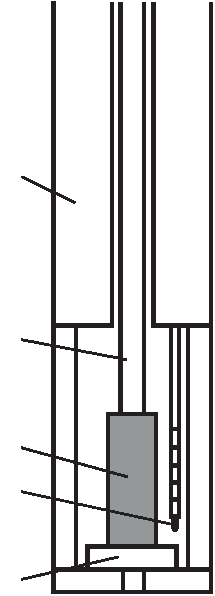
\includegraphics[width=\unitlength]{scheme_sample_measure}}%
        \put(0.08226702,1.93639265){\color[named]{black}\makebox(0,0)[rb]{\smash{\textsl{1}}}}%
        \put(0.07624028,1.1771024){\color[named]{black}\makebox(0,0)[rb]{\smash{\textsl{2}}}}%
        \put(0.0780196,0.65991058){\color[named]{black}\makebox(0,0)[rb]{\smash{\textsl{3}}}}%
        \put(0.07411657,0.44885082){\color[named]{black}\makebox(0,0)[rb]{\smash{\textsl{4}}}}%
        \put(0.07503493,0.033652){\color[named]{black}\makebox(0,0)[rb]{\smash{\textsl{5}}}}%
      \end{picture}%
    \endgroup%

    \caption{Схема размещения измеряемого образца в термомеханическом анализаторе~\cite{Sinev_Petrov2016_cte_glass}:}
    \label{fig:scheme_sample_measure}
    \textsl{1} "--- колба, \textsl{2} "--- зонд, \textsl{3} "--- измеряемый образец, \textsl{4} "--- термопара, \textsl{5} "--- пьедестал%
\end{figure}
Линейное приращение длины и длину образца при комнатной температуре измеряли с помощью зонда из кварцевого стекла, опирающегося на~образец с~силой 0,2~Н.
Перед началом измерений термокамеру анализатора охлаждали.
Последующий нагрев проводили со скоростью 10 K/мин.
Значения температуры и~линейного приращения длины регистрировались автоматически программным обеспечением термомеханического анализатора через равные промежутки времени.
Для каждого образца было получено по 20 экспериментальных точек в~интервале от~129 до~800~K с~шагом не менее 35 K.
По~окончании измерений для каждого образца проводили программную коррекцию искажений, вносимых материалом колбы и зонда, с использованием эталона боросиликатного стекла SRM731.

Аналогичным образом были исследованы образцы стёкол марок Corning~7740 и SD\nb-2  в диапазоне от 170 до 780~K (от минус 100 до 500~{\textdegree}C).

\subsection{Расчёт погрешностей}
Значения
температурных коэффициентов линейного расширения
$\alpha (T)$, 1/K, были рассчитаны следующим образом в соответствии с определением \mbox{ТКЛР}~\cites[150]{Mazurin1969_Tepl_rassh_stekla}[44]{novikova1974}:
\begin{equation}
  \alpha (T)=\frac{\Delta L}{L_0 \Delta T},
\end{equation}
\[
    T=\frac{T_i+T_{i+1}}{2},
\]
\[
    \Delta T=T_{i+1}-T_i,
\]
\[
    \Delta L=L(T_{i+1})-L(T_i),
\]
где $T$ "--- средняя температура между $i$ и $i+1$ измеренными значениями, K;  $\Delta L$ "--- разница между $i+1$ и $i$ измеренными значениями длины, м; $L_0$ "--- исходная длина образца при комнатной температуре $T_0 =$~293,15~K, м;  $\Delta T$ "--- разница между $i+1$ и $i$ измеренными значениями температуры, K; $T_i$ "--- $i$\nb-ое измеренное значение температуры, K; $L(T_i)$ "--- измеренное значение длины образца при температуре $T_i$, м.

Температурная зависимость относительного теплового удлинения образца,  $\epsilon^T(T_i)$, рассчитывалась по следующей формуле:

\begin{equation}
\epsilon^T(T_i)=\frac{L(T_i)-L_0}{L_0}
\end{equation}

Согласно~\cite{ref_gosreestr_tma_ss} для данной измерительной установки пределы допускаемой относительной погрешности измерений линейных приращений длины составляют ${\pm}$3~\%, пределы допускаемой абсолютной погрешности измерений температуры равны ${\pm}$1~{\textdegree}C.

Была проведена оценка относительных погрешностей косвенных измерений ТКЛР и относительного удлинения в точках их максимальных значений в рассматриваемом интервале температур.
По формуле~\eqref{eq:cte_uncertainty} была рассчитана относительная погрешность
ТКЛР согласно~\cites[58]{KassandrovaLebedev1970Obrabotka}:
\begin{equation}
    \label{eq:cte_uncertainty}
    \frac{\delta \alpha}{\alpha}=
    \sqrt{
        \left(
            \frac{\delta (\Delta L)}{\Delta L}
        \right)^{\!\!2} %притягиваем степень к скобкам
        +
        \left(
            \frac{\delta (\Delta T)}{\Delta T}
        \right)^{\!\!2} %притягиваем степень к скобкам
        +
        \left(
            \frac{\delta L_0}{L_0}
        \right)^{\!\!2} %притягиваем степень к скобкам
    },
\end{equation}
где относительные погрешности измерений:
$\frac{\delta (\Delta L)}{\Delta L}$ "--- линейных приращений длины;
$\frac{\delta (\Delta T)}{\Delta T}$ "--- разницы температур;
$\frac{\delta L_0}{L_0}$ "--- длины образца при комнатной температуре.

Значения относительной погрешности измерений линейных приращений длины были
взяты из данных, приведённых в~\cite{ref_gosreestr_tma_ss}. Относительная
погрешность измерений разницы температур была определена в соответствии
с~\cites[57]{KassandrovaLebedev1970Obrabotka} по~формуле:
\begin{equation}
    \frac{\delta (\Delta T)}{\Delta T}=\frac{\delta T\cdot \sqrt 2}{\Delta T},
\end{equation}
где  $\delta T$ "--- абсолютная погрешность измерений температуры, взятая из~\cite{ref_gosreestr_tma_ss}, а~в~качестве величины  $\Delta T$ было взято минимальное значение разницы температур из~всей последовательности измерений в заявленном температурном интервале.

Относительная погрешность измерений длины образца при комнатной температуре с
учётом данных по относительной погрешности измерений линейных приращений длины
измерительной установкой~\cite{ref_gosreestr_tma_ss} была определена
в~соответствии с~\cites[57]{KassandrovaLebedev1970Obrabotka} следующим образом:
\begin{equation}
    \label{eq:otn_deltaL0}
    \frac{\delta L_0}{L_0}=\frac{\delta (\Delta L)}{\Delta L}\cdot \frac{\Delta L}{\sqrt 2L_0},
\end{equation}
где в качестве величины  $\Delta L$ было взято максимальное значение удлинений образца из всей последовательности измерений в заявленном температурном интервале.

В формуле~\eqref{eq:elongation_uncertainty} приведена оценка относительной
погрешности измерения относительного удлинения образца
согласно~\cites[58]{KassandrovaLebedev1970Obrabotka}:
\begin{equation}
    \label{eq:elongation_uncertainty}
    \frac{\delta \epsilon^T}{\epsilon^T}
    =
    \sqrt{
        \left(
            \frac{\delta (\Delta L)}{\Delta L}
        \right)^{\!\!2} %притягиваем степень к скобкам
        +
        \left(
            \frac{\alpha \delta T}{\epsilon^T}
        \right)^{\!\!2} %притягиваем степень к скобкам
        +
        \left(
            \frac{\delta L_0}{L_0}
        \right)^{\!\!2} %притягиваем степень к скобкам
    },
\end{equation}
где выражение  $\displaystyle\frac{\alpha \delta T}{\epsilon^T}$ введено аналогично описанному в~\cite{LTEC_si_293_1000} для учёта зависимости  $\epsilon^T$ от температуры. В нём использованы расчётные значения  $\alpha$ и  $\epsilon^T$ полученные из аппроксимации экспериментальных данных для температуры 800~K. Третий подкоренной элемент формулы~\eqref{eq:elongation_uncertainty} был рассчитан
по~формуле~\eqref{eq:otn_deltaL0}, но в качестве  $\Delta L$ было принято:
\begin{equation}
    \Delta L=\epsilon^T\cdot L_0.
\end{equation}

Относительная погрешность косвенных измерений ТКЛР стёкол, рассчитанная по
формуле~\eqref{eq:cte_uncertainty}, не превышает ${\pm}$5~\%.
Эта величина использована для отображения погрешности измерений на графиках на
Рисунках~\ref{fig:cte_bf33+official} и~\ref{fig:cte_lk5+official}.
Относительная погрешность косвенных измерений относительного удлинения стёкол,
рассчитанная по формуле~\eqref{eq:elongation_uncertainty}, не превышает
${\pm}$3~\%.

\subsection{Аппроксимация результатов полиномиальными функциями}
Функции, аппроксимирующие экспериментальные данные, получены методом наименьших квадратов. Данные функции имеют вид полиномов:
\begin{equation}\label{eq:polynom_sample}
    P(T) = a + b \cdot T + c \cdot T^2 + d \cdot T^3 + e \cdot T^4,
\end{equation}
где $a$, $b$, $c$, $d$, $e$ "--- коэффициенты полинома.

Результаты аппроксимации экспериментальных данных ТКЛР и относительного
теплового удлинения полиномами не выше 4-го порядка сведены
в~Таблицы~\ref{tab:results_approx_cte} и~\ref{tab:results_approx_rel_exp},
соответсвенно.

Полученные стандартные ошибки регрессий не превышают рассчитанных относительных
погрешностей косвенных измерений кроме аппроксимаций относительного удлинения в
интервале температур от~235 до~340~K. Кривые полученных зависимостей $\alpha(T)$
стёкол показаны на рисунках: Borofloat~33 "---
на~Рисунке~\ref{fig:cte_bf33+official}, ЛК5 "--- на Рисунке~\ref{fig:cte_lk5+official},
Hoya SD-2 "--- на Рисунке~\ref{fig:cte_SD-2+official}, Corning 7740 "---
на~Рисунке~\ref{fig:cte_7740+official}.

\begin{table} [!ht]
    \centering%
	\caption{Результаты аппроксимации экспериментальных значений температурной зависимости ТКЛР $\alpha (T)$, 1/K}%
	\label{tab:results_approx_cte}% label всегда желательно идти после caption
    \renewcommand{\arraystretch}{1.5}%% Увеличение расстояния между рядами, для улучшения восприятия.
    \sisetup{
        table-number-alignment = center,
    }%
	\begin{SingleSpace}
	\begin{tabularx}{\textwidth}{@{}
	>{\raggedright}X
	S[table-format=1.3]
	S[table-format=1.3]
	S[table-format=-1.3]
	S[table-format=1.3]
	>{\raggedleft}m{0.069\textwidth}
	>{\raggedleft}m{0.069\textwidth}
	>{\raggedleft\arraybackslash}m{0.069\textwidth}
	@{}%
	}
        \toprule     %%% верхняя линейка
        Марка стекла &
        {$a$, 10\textsuperscript{$-$6}} &
        {$b$, 10\textsuperscript{$-$8}} &
        {$c$, 10\textsuperscript{$-$11}}&
        {$d$, 10\textsuperscript{$-$14}}&
        {RSS, 10\textsuperscript{$-$14}} &
        {MSE, 10\textsuperscript{$-$15}} &
        {SER, 10\textsuperscript{$-$8}}\\
        \midrule
        Corning~7740 &
        2,893 &
        0,500 &
        -1,231 &
        0,740 &
        23,0 &
        14,0 &
        12,0\\
        Schott Borofloat~33 &
        1,628 &
        1,040 &
        -2,198 &
        1,398 &
        5,9 &
        3,9 &
        6,2\\
        ЛК5 &
        1,123 &
        1,607 &
        -3,496 &
        2,435 &
        25,0 &
        17,0 &
        13,0\\
        Hoya SD\nobreakdash-2 &
        -0,193 &
        1,453 &
        -1,847 &
        0,910 &
        9,8 &
        5,5 &
        7,4\\
        \bottomrule %%% нижняя линейка
	\end{tabularx}%
	\end{SingleSpace}
\end{table}

\begin{table} [ht]
    \centering%
	\caption{Результаты аппроксимации экспериментальных значений температурной зависимости относительного удлинения $\epsilon^T (T)$}%
	\label{tab:results_approx_rel_exp}% label всегда желательно идти после caption
    \renewcommand{\arraystretch}{1.6}%% Увеличение расстояния между рядами, для улучшения восприятия.
	\def\tabularxcolumn#1{m{#1}}
    \sisetup{
        table-number-alignment = center,
    }%
	\begin{SingleSpace}
	\begin{tabularx}{0.998\textwidth}{@{}
	>{\raggedright}X
	S[table-format=-1.3]
	S[table-format=-1.3]
	S[table-format=1.3]
	S[table-format=-1.3]
	S[table-format=1.3]
	>{\raggedleft}m{0.0686\textwidth}
	>{\raggedleft}m{0.0686\textwidth}
	>{\raggedleft\arraybackslash}m{0.0686\textwidth}
	@{}}
        \toprule     %%% верхняя линейка
        Марка стекла &
        {$a$, 10\textsuperscript{$-$4}} &
        {$b$, 10\textsuperscript{$-$6}} &
        {$c$, 10\textsuperscript{$-$9}}&
        {$d$, 10\textsuperscript{$-$12}}&
        {$e$, 10\textsuperscript{$-$15}}&
        {RSS, 10\textsuperscript{$-$11}} &
        {MSE, 10\textsuperscript{$-$12}} &
        {SER, 10\textsuperscript{$-$6}}\\
        \midrule
        Corning 7740 &
        -10,015 &
          3,297 &
          0,782 &
        -1,196 &
         0,139 &
        60,0 &
        36,0 &
        6,0\\
        Schott Borofloat 33 &
        -7,468 &
        1,451 &
        5,880 &
        -8,426 &
        4,136 &
        4,8 &
        3,2 &
        1,8\\
        ЛК5 &
        -7,494 &
        0,957 &
        8,460 &
        -12,080 &
        6,246 &
        36,0 &
        24,0 &
        4,9\\
        Hoya SD\nobreakdash-2 &
        -4,208 &
        -0,292 &
        7,691 &
        -6,860 &
        2,657 &
        16,0 &
        9,1 &
        3,0\\
        \bottomrule %%% нижняя линейка
	\end{tabularx}%
	\end{SingleSpace}
\end{table}

\begin{samepage}
\begin{figure}[!ht]
    \centering
    \begingroup%
      \makeatletter%
      \providecommand\color[2][]{%
        \errmessage{(Inkscape) Color is used for the text in Inkscape, but the package 'color.sty' is not loaded}%
        \renewcommand\color[2][]{}%
      }%
      \providecommand\transparent[1]{%
        \errmessage{(Inkscape) Transparency is used (non-zero) for the text in Inkscape, but the package 'transparent.sty' is not loaded}%
        \renewcommand\transparent[1]{}%
      }%
      \providecommand\rotatebox[2]{#2}%
      \ifx\svgwidth\undefined%
        \setlength{\unitlength}{0.5\textwidth}%
        \ifx\svgscale\undefined%
          \relax%
        \else%
          \setlength{\unitlength}{\unitlength * \real{\svgscale}}%
        \fi%
      \else%
        \setlength{\unitlength}{\svgwidth}%
      \fi%
      \global\let\svgwidth\undefined%
      \global\let\svgscale\undefined%
      \makeatother%
      \begin{picture}(1,0.69801469)%
        \put(0,0){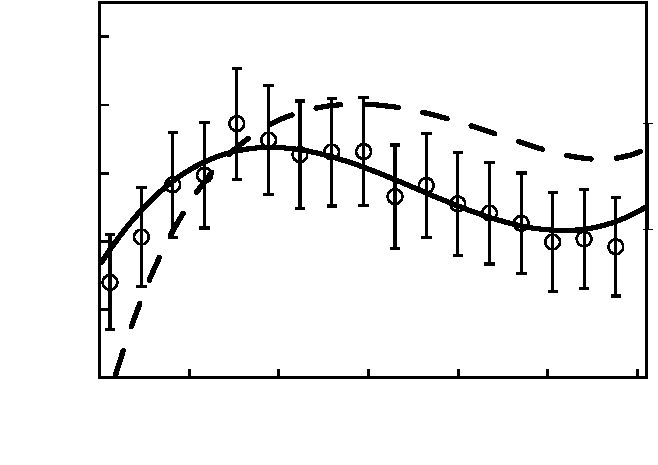
\includegraphics[width=\unitlength]{cte_bf33+official}}%
        \put(0.05707158,0.11269191){\color[named]{black}\makebox(0,0)[lb]{\smash{2,5}}}%
        \put(0.05707158,0.21630763){\color[named]{black}\makebox(0,0)[lb]{\smash{2,7}}}%
        \put(0.05707158,0.31988995){\color[named]{black}\makebox(0,0)[lb]{\smash{2,9}}}%
        \put(0.05707158,0.42350566){\color[named]{black}\makebox(0,0)[lb]{\smash{3,1}}}%
        \put(0.05707158,0.52712137){\color[named]{black}\makebox(0,0)[lb]{\smash{3,3}}}%
        \put(0.05707158,0.63070369){\color[named]{black}\makebox(0,0)[lb]{\smash{3,5}}}%
        \put(0.11744589,0.06020709){\color[named]{black}\makebox(0,0)[lb]{\smash{170}}}%
        \put(0.253639,0.06020709){\color[named]{black}\makebox(0,0)[lb]{\smash{270}}}%
        \put(0.38983211,0.06020709){\color[named]{black}\makebox(0,0)[lb]{\smash{370}}}%
        \put(0.52605861,0.06020709){\color[named]{black}\makebox(0,0)[lb]{\smash{470}}}%
        \put(0.66225172,0.06020709){\color[named]{black}\makebox(0,0)[lb]{\smash{570}}}%
        \put(0.79844483,0.06020709){\color[named]{black}\makebox(0,0)[lb]{\smash{670}}}%
        \put(0.93463794,0.06020709){\color[named]{black}\makebox(0,0)[lb]{\smash{770}}}%
        \put(0.03073901,0.25971627){\color[named]{black}\rotatebox{90}{\makebox(0,0)[lb]{\smash{$\alpha$, $10^{-6}$ 1/K}}}}%
        \put(0.50717079,0.00737128){\color[named]{black}\makebox(0,0)[lb]{\smash{$T$, K}}}%
      \end{picture}%
    \endgroup%

    \caption{Аппроксимация и экспериментальные значения коэффициента теплового линейного расширения Borofloat 33:}
    \label{fig:cte_bf33+official}
    Штриховая линия "--- аппроксимация данных производителя
\end{figure}

\begin{figure}[!hb]
    \centering
    \begingroup%
      \makeatletter%
      \providecommand\color[2][]{%
        \errmessage{(Inkscape) Color is used for the text in Inkscape, but the package 'color.sty' is not loaded}%
        \renewcommand\color[2][]{}%
      }%
      \providecommand\transparent[1]{%
        \errmessage{(Inkscape) Transparency is used (non-zero) for the text in Inkscape, but the package 'transparent.sty' is not loaded}%
        \renewcommand\transparent[1]{}%
      }%
      \providecommand\rotatebox[2]{#2}%
      \ifx\svgwidth\undefined%
        \setlength{\unitlength}{0.5\textwidth}%
        \ifx\svgscale\undefined%
          \relax%
        \else%
          \setlength{\unitlength}{\unitlength * \real{\svgscale}}%
        \fi%
      \else%
        \setlength{\unitlength}{\svgwidth}%
      \fi%
      \global\let\svgwidth\undefined%
      \global\let\svgscale\undefined%
      \makeatother%
      \begin{picture}(1,0.76900229)%
        \put(0,0){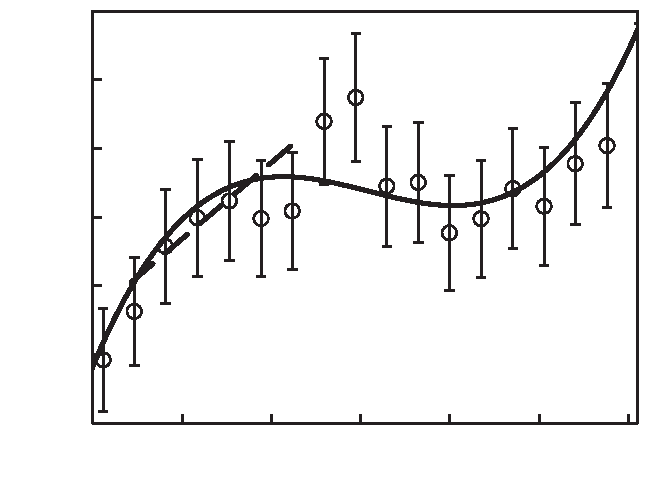
\includegraphics[width=\unitlength]{cte_lk5+official}}%
        \put(0.05896161,0.10384021){\color[named]{black}\makebox(0,0)[lb]{\smash{2,8}}}%
        \put(0.05896161,0.20966433){\color[named]{black}\makebox(0,0)[lb]{\smash{3,0}}}%
        \put(0.05896161,0.31545445){\color[named]{black}\makebox(0,0)[lb]{\smash{3,2}}}%
        \put(0.05896161,0.42124457){\color[named]{black}\makebox(0,0)[lb]{\smash{3,4}}}%
        \put(0.05896161,0.52706876){\color[named]{black}\makebox(0,0)[lb]{\smash{3,6}}}%
        \put(0.05896161,0.63285888){\color[named]{black}\makebox(0,0)[lb]{\smash{3,8}}}%
        \put(0.05896161,0.73864897){\color[named]{black}\makebox(0,0)[lb]{\smash{4,0}}}%
        \put(0.1090145,0.05902576){\color[named]{black}\makebox(0,0)[lb]{\smash{170}}}%
        \put(0.24651103,0.05902576){\color[named]{black}\makebox(0,0)[lb]{\smash{270}}}%
        \put(0.38399049,0.05902576){\color[named]{black}\makebox(0,0)[lb]{\smash{370}}}%
        \put(0.52147002,0.05902576){\color[named]{black}\makebox(0,0)[lb]{\smash{470}}}%
        \put(0.65896647,0.05902576){\color[named]{black}\makebox(0,0)[lb]{\smash{570}}}%
        \put(0.79644601,0.05902576){\color[named]{black}\makebox(0,0)[lb]{\smash{670}}}%
        \put(0.93397646,0.05902576){\color[named]{black}\makebox(0,0)[lb]{\smash{770}}}%
        \put(0.0311866,0.26509523){\color[named]{black}\rotatebox{90}{\makebox(0,0)[lb]{\smash{$\alpha$, $10^{-6}$ 1/K}}}}%
        \put(0.53009853,0.00747856){\color[named]{black}\makebox(0,0)[lb]{\smash{$T$, K}}}%
      \end{picture}%
    \endgroup%

    \caption{Аппроксимация и экспериментальные значения коэффициента теплового линейного расширения ЛК5:}
    \label{fig:cte_lk5+official}
    Штриховая линия "--- аппроксимация данных производителя
\end{figure}
\end{samepage}

\begin{samepage}
\begin{figure}[!htb]
    \centering
    \begingroup%
      \makeatletter%
      \providecommand\color[2][]{%
        \errmessage{(Inkscape) Color is used for the text in Inkscape, but the package 'color.sty' is not loaded}%
        \renewcommand\color[2][]{}%
      }%
      \providecommand\transparent[1]{%
        \errmessage{(Inkscape) Transparency is used (non-zero) for the text in Inkscape, but the package 'transparent.sty' is not loaded}%
        \renewcommand\transparent[1]{}%
      }%
      \providecommand\rotatebox[2]{#2}%
      \ifx\svgwidth\undefined%
        \setlength{\unitlength}{0.5\textwidth}%
        \ifx\svgscale\undefined%
          \relax%
        \else%
          \setlength{\unitlength}{\unitlength * \real{\svgscale}}%
        \fi%
      \else%
        \setlength{\unitlength}{\svgwidth}%
      \fi%
      \global\let\svgwidth\undefined%
      \global\let\svgscale\undefined%
      \makeatother%
      \begin{picture}(1,0.73146883)%
        \put(0,0){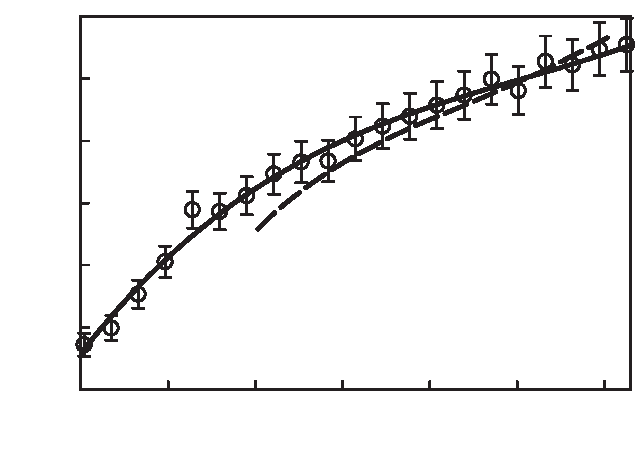
\includegraphics[width=\unitlength]{cte_SD-2+official}}%
        \put(0.52181269,0.00655847){\color[named]{black}\makebox(0,0)[lb]{\smash{$T$, K}}}%
        \put(0.02734947,0.2858294){\color[named]{black}\rotatebox{90}{\makebox(0,0)[lb]{\smash{$\alpha$, $10^{-6}$ 1/K}}}}%
        \put(0.04882056,0.1174594){\color[named]{black}\makebox(0,0)[lb]{\smash{1,5}}}%
        \put(0.05321852,0.21461843){\color[named]{black}\makebox(0,0)[lb]{\smash{2,0}}}%
        \put(0.05321852,0.31177746){\color[named]{black}\makebox(0,0)[lb]{\smash{2,5}}}%
        \put(0.05234342,0.40893649){\color[named]{black}\makebox(0,0)[lb]{\smash{3,0}}}%
        \put(0.05234342,0.50609572){\color[named]{black}\makebox(0,0)[lb]{\smash{3,5}}}%
        \put(0.05348779,0.60325475){\color[named]{black}\makebox(0,0)[lb]{\smash{4,0}}}%
        \put(0.05348779,0.70041378){\color[named]{black}\makebox(0,0)[lb]{\smash{4,5}}}%
        \put(0.09083587,0.064941){\color[named]{black}\makebox(0,0)[lb]{\smash{170}}}%
        \put(0.23102922,0.064941){\color[named]{black}\makebox(0,0)[lb]{\smash{270}}}%
        \put(0.36858599,0.064941){\color[named]{black}\makebox(0,0)[lb]{\smash{370}}}%
        \put(0.50715254,0.064941){\color[named]{black}\makebox(0,0)[lb]{\smash{470}}}%
        \put(0.64440638,0.064941){\color[named]{black}\makebox(0,0)[lb]{\smash{570}}}%
        \put(0.78251299,0.064941){\color[named]{black}\makebox(0,0)[lb]{\smash{670}}}%
        \put(0.92064194,0.064941){\color[named]{black}\makebox(0,0)[lb]{\smash{770}}}%
      \end{picture}%
    \endgroup%

    \caption{Аппроксимация и экспериментальные значения коэффициента теплового линейного расширения Hoya SD-2:}
    \label{fig:cte_SD-2+official}
    Штриховая линия "--- аппроксимация данных производителя
\end{figure}

\begin{figure}[!htb]
    \centering
    \begingroup%
      \makeatletter%
      \providecommand\color[2][]{%
        \errmessage{(Inkscape) Color is used for the text in Inkscape, but the package 'color.sty' is not loaded}%
        \renewcommand\color[2][]{}%
      }%
      \providecommand\transparent[1]{%
        \errmessage{(Inkscape) Transparency is used (non-zero) for the text in Inkscape, but the package 'transparent.sty' is not loaded}%
        \renewcommand\transparent[1]{}%
      }%
      \providecommand\rotatebox[2]{#2}%
      \ifx\svgwidth\undefined%
        \setlength{\unitlength}{0.5\textwidth}%
        \ifx\svgscale\undefined%
          \relax%
        \else%
          \setlength{\unitlength}{\unitlength * \real{\svgscale}}%
        \fi%
      \else%
        \setlength{\unitlength}{\svgwidth}%
      \fi%
      \global\let\svgwidth\undefined%
      \global\let\svgscale\undefined%
      \makeatother%
      \begin{picture}(1,0.71082807)%
        \put(0,0){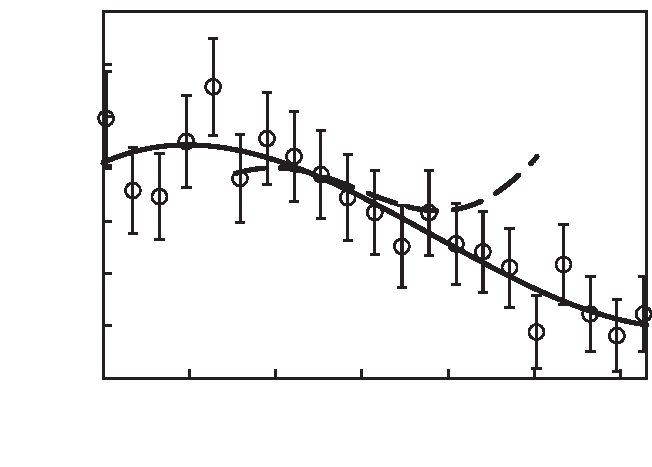
\includegraphics[width=\unitlength]{cte_7740+official}}%
        \put(0.06109288,0.11853542){\color[named]{black}\makebox(0,0)[lb]{\smash{2,6}}}%
        \put(0.06109288,0.1988594){\color[named]{black}\makebox(0,0)[lb]{\smash{2,8}}}%
        \put(0.06109288,0.27913159){\color[named]{black}\makebox(0,0)[lb]{\smash{3,0}}}%
        \put(0.06109288,0.35945557){\color[named]{black}\makebox(0,0)[lb]{\smash{3,2}}}%
        \put(0.06109288,0.43972776){\color[named]{black}\makebox(0,0)[lb]{\smash{3,4}}}%
        \put(0.06109288,0.51999994){\color[named]{black}\makebox(0,0)[lb]{\smash{3,6}}}%
        \put(0.06109288,0.60032392){\color[named]{black}\makebox(0,0)[lb]{\smash{3,8}}}%
        \put(0.06109288,0.68059611){\color[named]{black}\makebox(0,0)[lb]{\smash{4,0}}}%
        \put(0.12343288,0.06432454){\color[named]{black}\makebox(0,0)[lb]{\smash{170}}}%
        \put(0.25581035,0.06432454){\color[named]{black}\makebox(0,0)[lb]{\smash{270}}}%
        \put(0.38815334,0.06432454){\color[named]{black}\makebox(0,0)[lb]{\smash{370}}}%
        \put(0.52054813,0.06432454){\color[named]{black}\makebox(0,0)[lb]{\smash{470}}}%
        \put(0.6529256,0.06432454){\color[named]{black}\makebox(0,0)[lb]{\smash{570}}}%
        \put(0.78530307,0.06432454){\color[named]{black}\makebox(0,0)[lb]{\smash{670}}}%
        \put(0.91769787,0.06432454){\color[named]{black}\makebox(0,0)[lb]{\smash{770}}}%
        \put(0.031062,0.2772676){\color[named]{black}\rotatebox{90}{\makebox(0,0)[lb]{\smash{$\alpha$, $10^{-6}$ 1/K}}}}%
        \put(0.53822139,0.00744878){\color[named]{black}\makebox(0,0)[lb]{\smash{$T$, K}}}%
      \end{picture}%
    \endgroup%

    \caption{Аппроксимация и экспериментальные значения коэффициента теплового линейного расширения Corning 7740:}
    \label{fig:cte_7740+official}
    Штриховая линия "--- аппроксимация данных производителя
\end{figure}
\end{samepage}

\subsection{Сравнение с данными производителей}
Сравним данные производителей по средним ТКЛР со средними значениями на тех же температурных интервалах рассчитанными по полученным аппроксимациям.

Средний ТКЛР стекла марки ЛК5 по полученным экспериментальным данным в диапазонах от минус 60 до плюс 20~{\textdegree}C и от 20 до 120~{\textdegree}C  совпадает с~данными производителя~\cite{LK5_properties}.

Средний ТКЛР стекла марки Borofloat 33 в диапазоне от 20 до 300~{\textdegree}C по~данным производителя~\cite{bf33_properties} составляет 3,25$\:\cdot\:$10\textsuperscript{$-$6}~1/${}^\circ$C, по полученным данным "--- 3,12$\:\cdot\:$10\textsuperscript{$-$6}~1/${}^\circ$C. Такое различие укладывается в погрешность проведённых измерений.

Средний ТКЛР стекла марки Corning 7740 в диапазоне от 0 до 300~{\textdegree}C по~данным производителя~\cite{corning7740_wafersheet} составляет 3,25$\:\cdot\:$10\textsuperscript{$-$6}~1/${}^\circ$C, по полученным данным "--- 3,34$\:\cdot\:$10\textsuperscript{$-$6}~1/${}^\circ$C. Такое различие укладывается в погрешность проведённых измерений.

Средний ТКЛР стекла марки Hoya SD\nb-2 в диапазоне от 20 до 300~{\textdegree}C по~данным производителя~\cite{SD_2_properties} составляет 3,20$\:\cdot\:$10\textsuperscript{$-$6}~1/${}^\circ$C, по полученным данным "--- 3,33$\:\cdot\:$10\textsuperscript{$-$6}~1/${}^\circ$C. Такое различие укладывается в погрешность проведённых измерений.

\clearpage
\section{Выводы по главе 2}

\begin{enumerate}
\setlist{midpenalty=5000}
    \item Исследован состав образцов четырёх марок стёкол, применяемых в
    отечественной и мировой практике для соединения с кремнием: Borofloat~33,
    Corning~7740, ЛК5 и~Hoya~SD\nb-2.
    Это позволит сопоставить данные, полученные в~этой работе,
    с~исследованиями других авторов.
    \item Анализ погрешностей проведённых измерений ТКЛР в
    диапазоне от~170 до 780~K (от минус 100 до
    500~{\textdegree}C) показал, что относительная погрешность
    измерений не превышает ${\pm}$5~\%.
    Полученные стандартные ошибки регрессий не превышают
    рассчитанные относительные погрешности.
    \item Сравнение с данными производителей по средним ТКЛР
    в диапазоне от~20 до 300~{\textdegree}C показало расхождение
    не превышающее погрешность проведённых измерений.
\end{enumerate}
